\documentclass{beamer}

% theme definition
\usetheme{KU}

\usepackage{natbib}
\usepackage{alltt}
\usepackage{trust}

\setbeamertemplate{blocks}[rounded][shadow=true]

\setbeamercolor{title}{fg=kublue}
\setbeamercolor{subtitle}{fg=kugray} 
\setbeamercolor{institute}{fg=kugray}
\setbeamercolor{frametitle}{fg=kublue}
\setbeamercolor{frametitle}{bg=white}
\setbeamercolor{framesubtitle}{fg=kugray}
\setbeamercolor{framesubtitle}{bg=white}
\setbeamercolor{item}{fg=black}
\setbeamercolor{subitem}{fg=kugray}
\setbeamercolor{itemize/enumerate subbody}{fg=kugray}
\setbeamercolor{block title}{bg=kublue}
\setbeamercolor{block title}{fg=white}
\setbeamercolor{block body}{bg=sand}
\setbeamercolor{block body}{fg=black}

\usefonttheme{serif}

\newenvironment{fnverbatim}{\begin{alltt}\scriptsize}{\normalsize\end{alltt}}
\newcommand{\mean}[1]{\langle#1\rangle}
\newcommand{\rtime}{\ensuremath{\mathbb{R}^{0\leq}}}

\bibliographystyle{abbrv}

\title{Trust}
\subtitle{What it is and how to get it}

\author{Dr. Perry Alexander}

%\date{{\color{kugray}\today}}
\date{\ }

% turns off navigation symbols
\setbeamertemplate{navigation symbols}{}

\institute{
    Information and Telecommunication Technology Center \\
    Electrical Engineering and Computer Science \\
    The University of Kansas \\
    \texttt{palexand@ku.edu}}

\begin{document}

\begin{frame}
  \titlepage

{\footnotesize\color{kugray} Formatted with the Beamer Class for \LaTeXe}
\end{frame}

\frame{\frametitle{Defining Trust}
  \begin{block}{Trust}
    ``An entity can be trusted if it always behaves in the expected
    manner for the intended purpose~\cite{Martin:08:The-ten-page-in}''
  \end{block}
}

\frame{\frametitle{Defining Trust}
  \begin{block}{Properties}
    \begin{itemize}
    \item Unambiguous identification
    \item Unimpeded operation
    \item First-hand observation of good behavior \emph{or} indirect
      experience of good behavior by a trusted third party
    \end{itemize}
  \end{block}
}

\frame{\frametitle{Necessary Capabilities for Trust}
  \begin{itemize}
  \item \emph{Strong Identification} --- An unambiguous, immutable
    identifier associated with the platform.  The identifier is a
    protected encryption key in the TXT implementation.
  \item \emph{Reporting Configuration} --- An unambiguous
    identification mechanism for software and hardware running on the
    platform.  The mechanism is hashing in the TXT implementation
  \end{itemize}
}

\frame{\frametitle{Tools for Trust}
  \begin{itemize}
  \item $\hash{X}$ --- Hash function such as MD-5
    \begin{itemize}
    \item $\hash{X}$ is unique for each $X$
    \item Guessing $X$ from $\hash{X}$ is impossible
    \end{itemize}
  \item $\encrypt{X}{Y}$ --- Encrypting $X$ with $Y$
    \begin{itemize}
    \item $X$ cannot be obtained from $\encrypt{X}{Y}$ without $Y$
    \item $Y$ cannot be guessed
    \end{itemize}
  \end{itemize}
}

\frame{\frametitle{Measurement --- Chaining Evidence}
  
  We would like to start $A$ and $B$ while gathering evidence of trust

    \begin{columns}[c]
    \column{.53\textwidth}
    \begin{itemize}
    \item<1-> Start with a root measurer and store that are trusted
      \emph{a priori}
    \item<2-> Measure the new software to be launched
    \item<3-> Store the measurement of the new software
    \item<4-> Launch the new software
    \item<5-> Repeat for each system software component
    \end{itemize}
    \column{.45\textwidth}
    \begin{figure}
      \only<1>{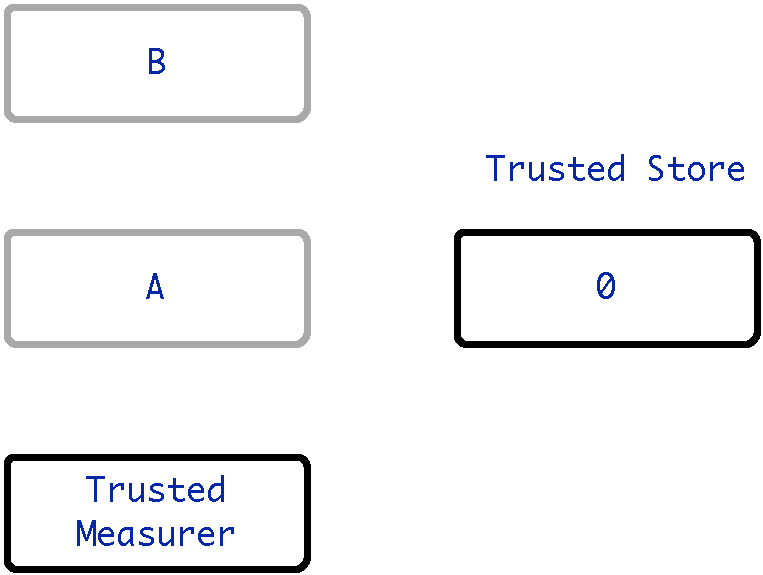
\includegraphics[width=1.0\textwidth]{figures/chain-root.pdf}}
      \only<2>{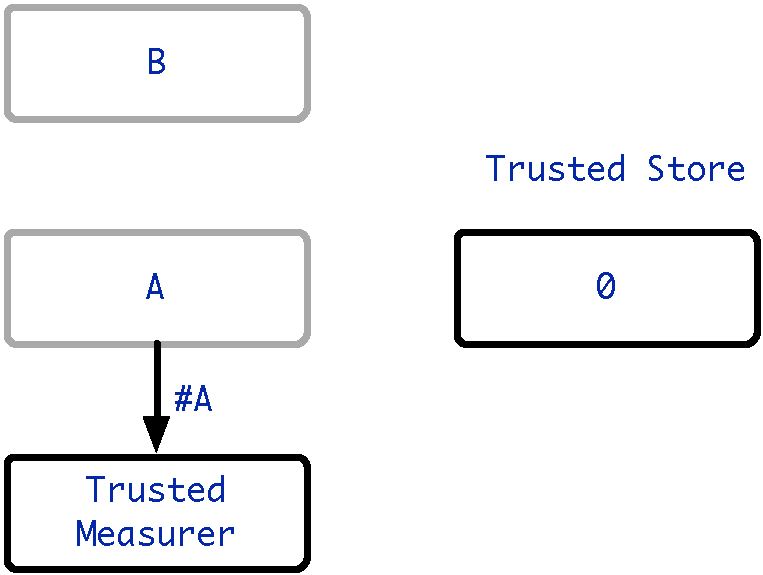
\includegraphics[width=1.0\textwidth]{figures/chain-measure.pdf}}
      \only<3>{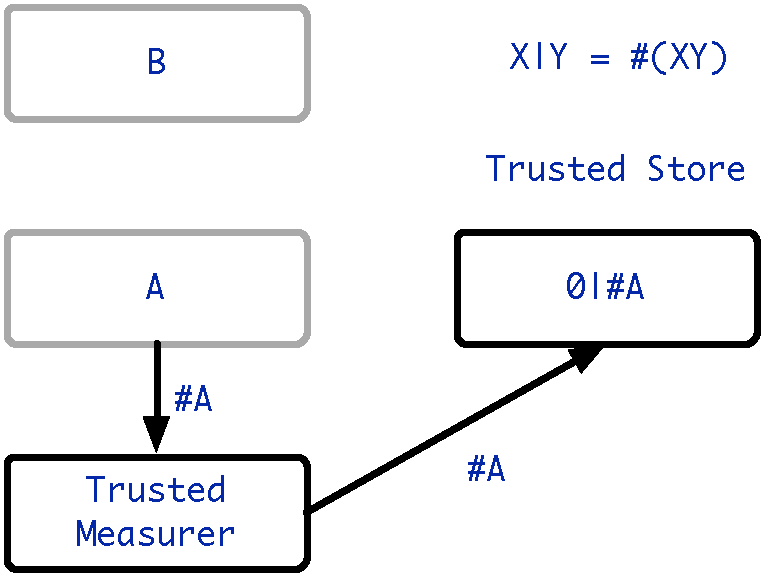
\includegraphics[width=1.0\textwidth]{figures/chain-store.pdf}}
      \only<4>{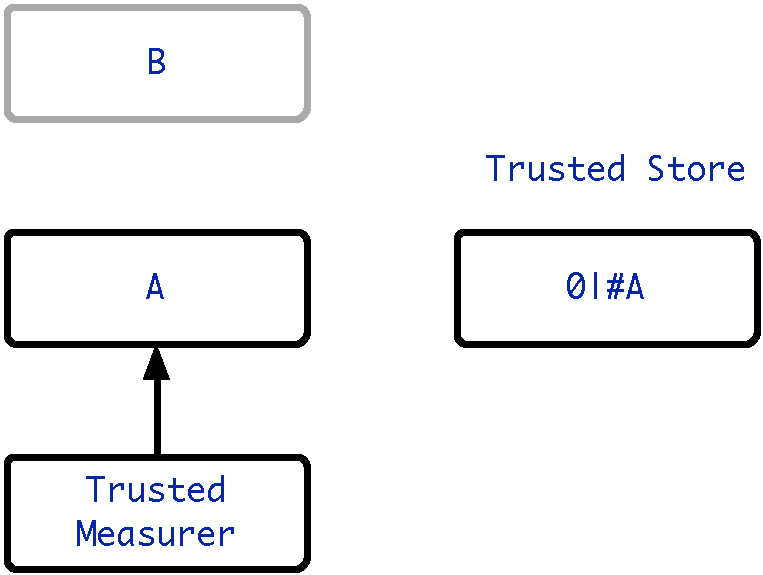
\includegraphics[width=1.0\textwidth]{figures/chain-start.pdf}}
      \only<5>{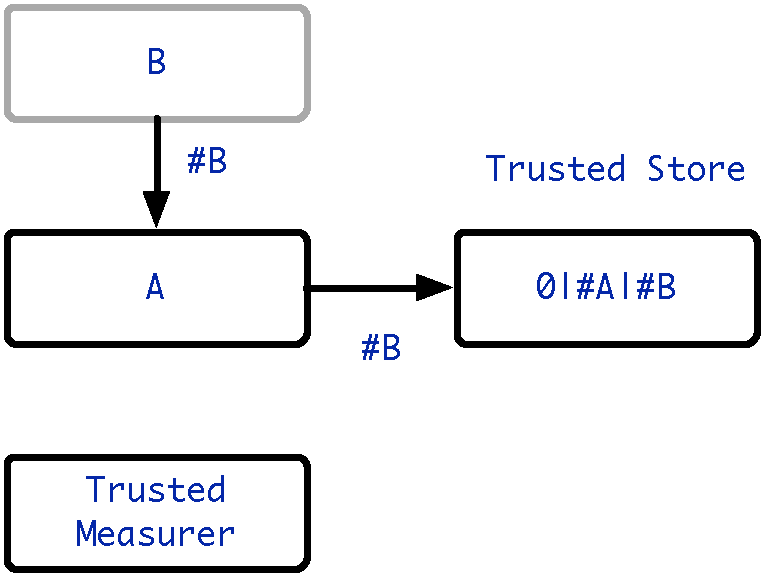
\includegraphics[width=1.0\textwidth]{figures/chain-next.pdf}}
      \only<6>{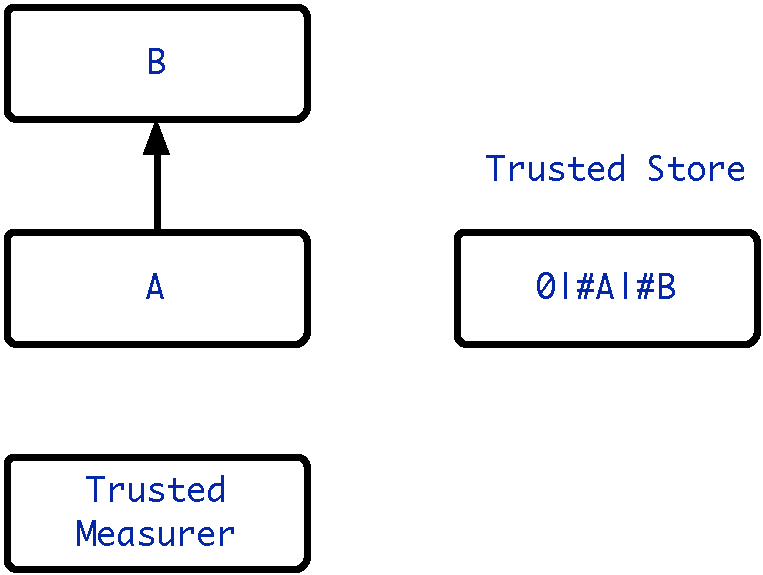
\includegraphics[width=1.0\textwidth]{figures/chain-final.pdf}}
    \end{figure}
  \end{columns}
}

\frame{\frametitle{Appraisal --- What Do We Know?}

  Measurement $\neq$ trust --- Measurements must be appraised

  \begin{itemize}
  \item Determine if $\extend{\extend{0}{\hash{A}}}{\hash{B}}$ is correct
    \begin{itemize}
    \item Calculate a \emph{golden hash} from $A$ and $B$
    \item Compare golden hash with
      $\extend{\extend{0}{\hash{A}}}{\hash{B}}$ from trusted store
    \item Correct $\extend{\extend{0}{\hash{A}}}{\hash{B}}$ implies
      trusted boot
    \end{itemize}
  \item Correct $\extend{\extend{0}{\hash{A}}}{\hash{B}}$ implies $A$ and $B$ must be correct
    \begin{itemize}
    \item Correct $\extend{\extend{0}{\hash{A}}}{\hash{B}}$ implies $\hash{A}$ and $\hash{B}$ are the correct hashes
    \item Correct $\hash{A}$ and $\hash{B}$ implies $A$ and $B$ are the correct binaries
    \item $A$ includes hash and launch functions
    \end{itemize}
  \item Correct $\extend{\extend{0}{\hash{A}}}{\hash{B}}$ implies measurement occurred in the right order
    \begin{itemize}
    \item $\hash{(XY)}\neq\hash{(YX)}$
    \item Trusted store started with 0
    \end{itemize}
  \end{itemize}
}

\frame{\frametitle{Appraisal --- But Why Trust B?}
  
  A chain exists from the Trusted Measurer and Trusted Store to B

  \begin{itemize}
  \item Trusted Measurer and Trusted Store are trusted \emph{a priori}
  \item $A$ is trusted to be $A$ because its measurement is:
    \begin{itemize}
    \item Correct
    \item Taken by a trusted party (Trusted Measurer)
    \item Stored by a trusted party (Trusted Store)
    \end{itemize}
  \item B is trusted to be B because its measurement is:
    \begin{itemize}
    \item Correct
    \item Taken by a trusted party (A)
    \item Stored by a trusted party (Trusted Store)
    \item If A's ability to measure B were compromised, $\hash{A}$
      would be wrong
    \end{itemize}
  \item and so on and so on...
  \end{itemize}
}

\frame{\frametitle{Trust is a Preorder}

  $\trusts{x}{y}$ is an homogeneous relation over actors that is true
  when \emph{x trusts y}.  $\trusts{x}{y}$ is a preorer:

  \begin{itemize}
  \item Reflexive - $\forall x \cdot \trusts{x}{x}$
  \item Transitive - $\forall x,y,z\cdot\trusts{x}{y}\wedge\trusts{y}{z}  \Rightarrow
  \trusts{x}{z}$
  \end{itemize}

  \alert{Measured Boot gathers evidence of these chains}
}


\frame{\frametitle{Trusted Platform Module}
  The \emph{Trusted Platform Module (TPM)} is a cryptographic
  coprocessor for trust.

  \begin{itemize}
  \item Endorsement Key (EK) --- factory generated asymmetric key
    that uniquely identifies the TPM
  \item Attestation Instance Key (AIK) ---
    \texttt{TPM\_CreateIdentity} generated asymmetric key alias for
    the EK
  \item Storage Root Key (SRK) --- \texttt{TPM\_TakeOwnership}
    generated asymmetric key that encrypts data associated with the
    TPM
  \item Platform Configuration Registers (PCRs) --- protected
    registers for storing and extending hashes
  \item NVRAM --- Non-volatile storage associated with the TPM
  \end{itemize}
}

\frame{\frametitle{Endorsement Key}
  \begin{itemize}
  \item Asymmetric key generated at TPM fabrication
  \item $\private{EK}$ is protected by the TPM
  \item $\public{EK}$ by convention is managed by a Certificate
    Authority
    \begin{itemize}
    \item Binds $\public{EK}$ with a platform
    \item Classic trusted third party
    \end{itemize}
  \item Only used for encryption
  \item Attestation Instance Keys (AIK) are aliases for the EK
    \begin{itemize}
    \item Used for signing
    \item Authorized by the EK
    \end{itemize}
  \end{itemize}
}

\frame{\frametitle{Storage Root Key}
  \begin{itemize}
  \item Asymmetric key generated by \texttt{TPM\_TakeOwnership}
  \item $\private{SRK}$ is protected by the TPM
  \item $\public{SRK}$ is available for encryption
  \item Used as the root for chaining keys by \emph{wrapping}
    \begin{itemize}
    \item A wrapped key is an asymmetric key pair with it's private
      key sealed
    \item Safe to share the entire key
    \item Only usable in the presence of the wrapping key with
      expected PCRs
    \end{itemize}
  \end{itemize}
}

\frame{\frametitle{Platform Configuration Registers}
  \begin{itemize}
  \item Operations on PCRs
    \begin{itemize}
    \item Extension --- Hash a new value juxtaposed with the existing
      PCR value
    \item Reset --- Set to 0
    \item Set --- Set to a known value
    \end{itemize}
  \item Operations using PCRs
    \begin{itemize}
    \item Sealing data --- PCR state dependent encryption
    \item Wrapping keys --- PCR state dependent encryption of a
      private key
    \item Quote --- Reporting PCR values to a third party
    \end{itemize}
  \item Properties
    \begin{itemize}
    \item Locality --- Access control
    \item Resettable --- Can a PCR be reset
    \item Many others that we don't need yet
    \end{itemize}
  \end{itemize}
}

\frame{\frametitle{Roots of Trust} 

  A \emph{root of trust} provides a basis for transitively building
  trust.  Roots of trust are trusted implicitly. 
  \\
  There are three important Roots of Trust:
  
  \begin{itemize}
  \item Root of Trust for Measurement (RTM)
  \item Root of Trust for Reporting (RTR)
  \item Root of Trust for Storage (RTS)
  \end{itemize}
}

\frame{\frametitle{Root of Trust for Measurement}
  A \emph{Root of Trust for Measurement} is trusted to take the base
  system measurement.

  \begin{itemize}
  \item A hash function called on an initial code base from
    a protected execution environment
  \item Starts the measurement process during boot
  \item In the Intel TXT process the RTM is \texttt{SENTER}
    implemented on the processor
  \end{itemize}
}

\frame{\frametitle{Root of Trust for Reporting}
  A \emph{Root of Trust for Reporting} is trusted to guarantee the
  integrity of the base system report or quote

  \begin{itemize}
  \item A protected key used for authenticating reports
  \item In the Intel TXT processes this is the TPM's Endorsement Key
    (EK)
  \item Created and bound to its platform by the TPM foundry
  \item $\private{EK}$ is stored in the TPM and cannot be accessed by
    any entity other than the TPM
  \item $\public{EK}$ is available for encrypting data for the TPM
  \item $\private{EK}$ is used for decrypting data inside the TPM
  \item Linking $\public{EK}$ to its platform is done by a trusted
    Certificate Authority (CA)
  \end{itemize}
}

\frame{\frametitle{Root of Trust for Storage}
  A \emph{Root of Trust for Storage} is trusted to protect stored data

  \begin{itemize}
  \item A key stored in a protected location
  \item In the Intel TXT boot process this is the TPM's Storage Root
    Key (SRK)
  \item Created by \texttt{TPM\_TakeOwnership}
  \item $\private{SRK}$ is stored in the TPM and cannot be accessed by
    any entity other than the TPM
  \item $\public{SRK}$ is available for encrypting data for the TPM
  \item SRK is used for protecting other keys
  \end{itemize}
}

\frame{\frametitle{One Step from Roots of Trust}
  
  Roots of trust are used to build a trusted system from boot.

  \begin{columns}[c]
    \column{.53\textwidth}
    \begin{itemize}
    \item<1-> Power-on reset
    \item<2-> Resettable PCRs set to -1
    \item<3-> \texttt{SENTER} called, resets resettable PCRs to 0
    \item<4-> \texttt{SENTER} measures \texttt{SINIT} policy into PCR 18
    \end{itemize}
    \column{.45\textwidth}
    \begin{figure}
      \only<1>{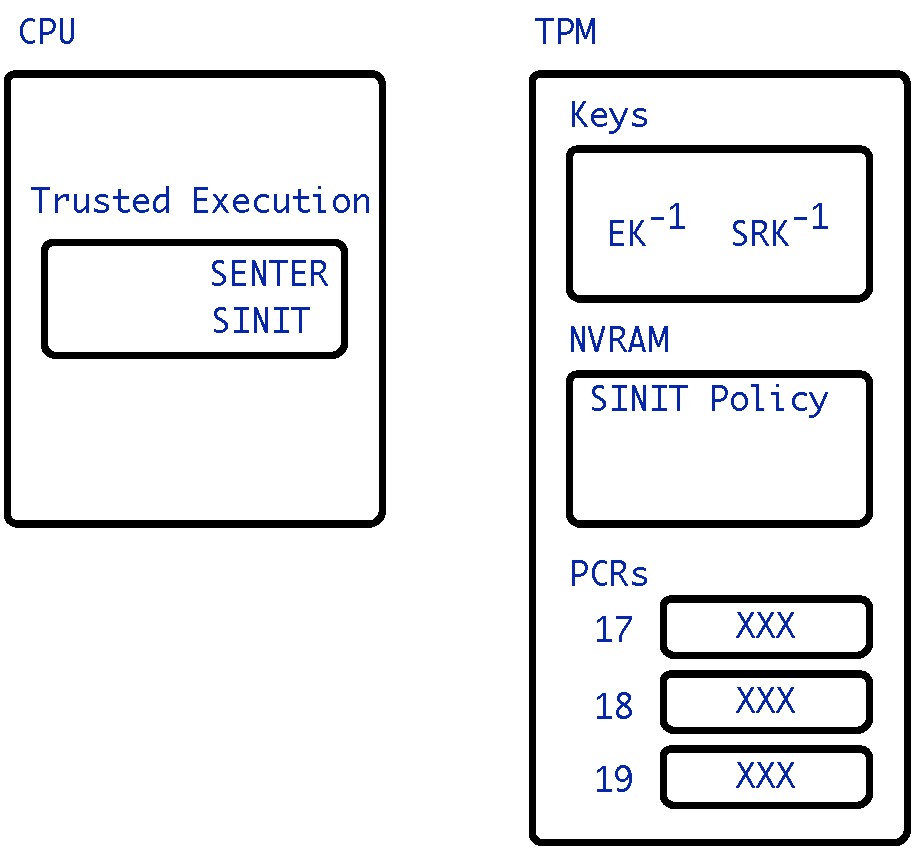
\includegraphics[width=1.0\textwidth]{figures/boot-pre-reset.pdf}}
      \only<2>{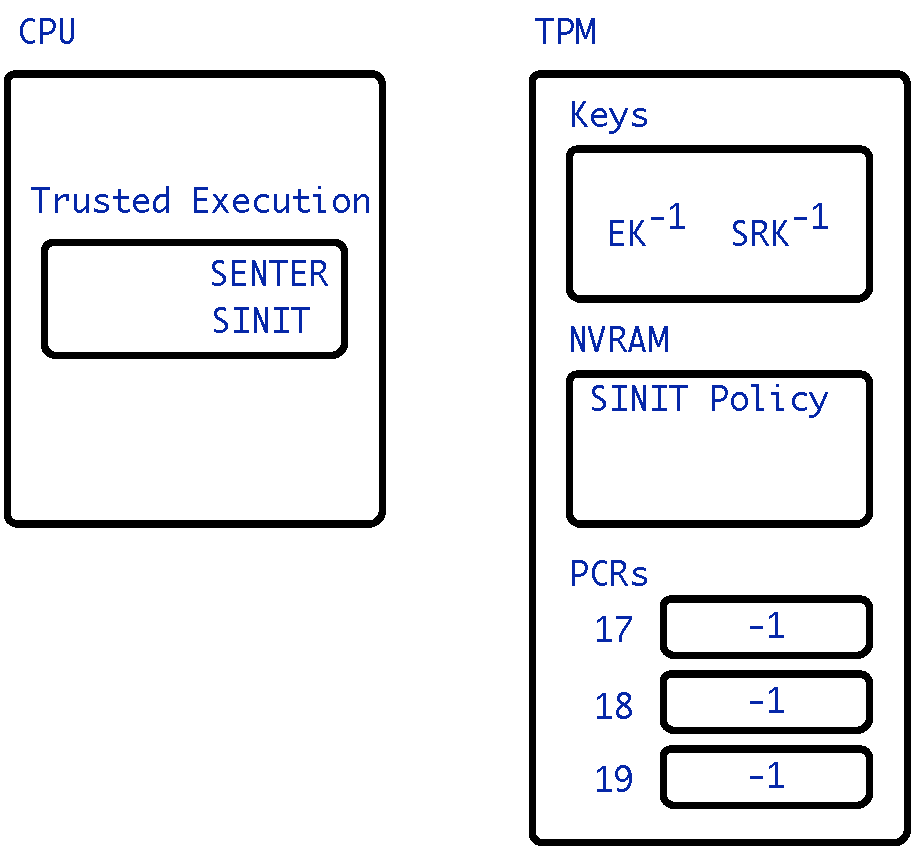
\includegraphics[width=1.0\textwidth]{figures/boot-reset.pdf}}
      \only<3>{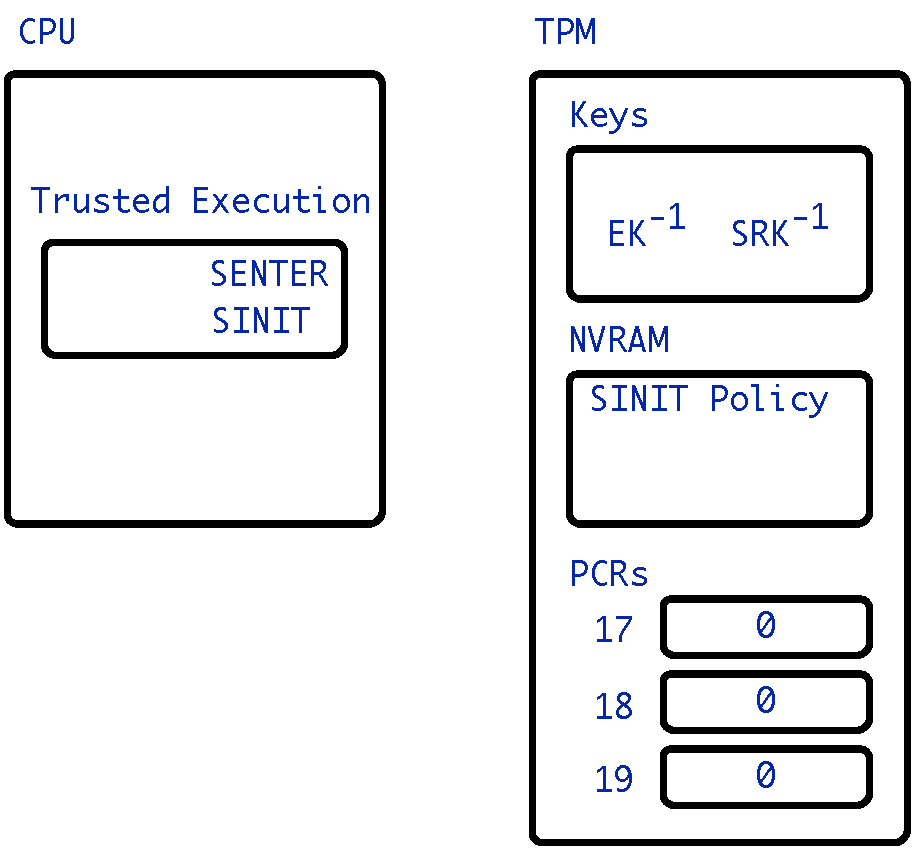
\includegraphics[width=1.0\textwidth]{figures/boot-senter.pdf}}
      \only<4>{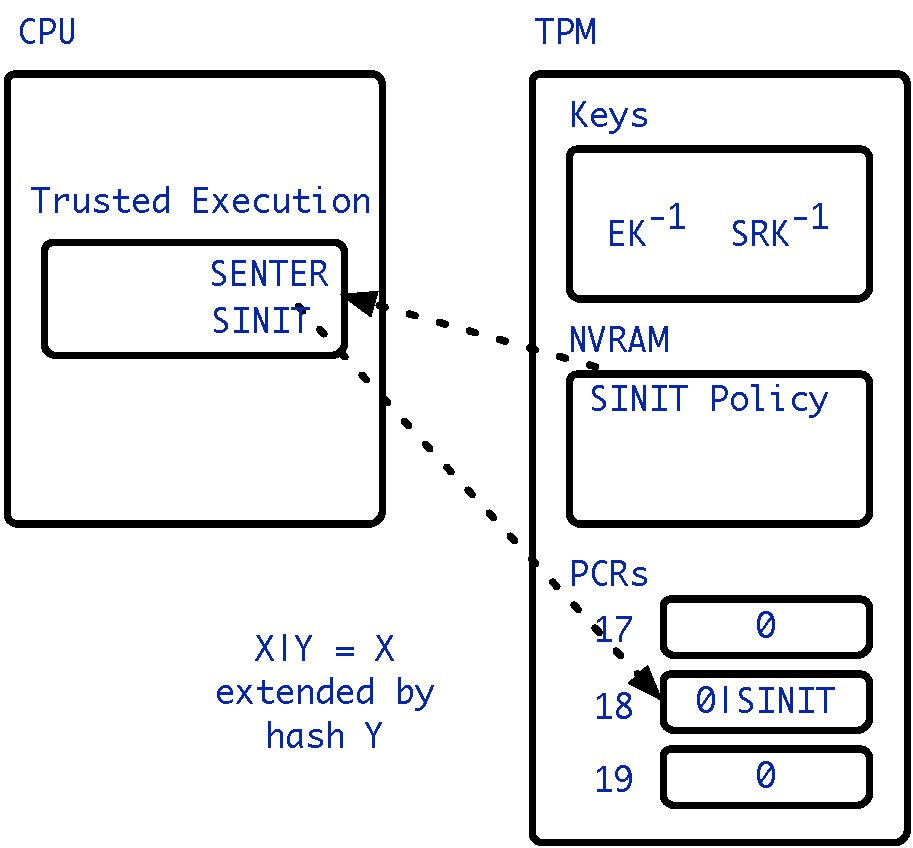
\includegraphics[width=1.0\textwidth]{figures/boot-senter-post.pdf}}
    \end{figure}
  \end{columns}
}

\frame{\frametitle{What We Know From Good PCR 18}
  A good value in PCR 18 tells us:

  \begin{itemize}
  \item \texttt{SENTER} was called --- Resetting PCR 18 starts
    measurements at 0 rather than -1
  \item \texttt{SINIT} was measured by \texttt{SENTER} --- Only
    \texttt{SENTER} can extend PCR 18
  \item \texttt{SINIT} uses the correct policy --- PCR 18 is extended
    with \texttt{SINIT} measurement policy
  \item \texttt{SENTER} ran before \texttt{SINIT} was measured ---
    $\extend{A}{B} \neq \extend{B}{A}$
  \end{itemize}

  \begin{block}{Measurement $\neq$ Trust}
    Measurements must be appraised to determine trust.
  \end{block}
}

\frame{\frametitle{Two Steps from Roots of Trust}

  \begin{columns}[c]
    \column{.53\textwidth}
    \begin{itemize}
    \item<1-> \texttt{SINIT} measures the Measured Launch Environment (MLE)
      using measured policy
    \item<1-> \texttt{SINIT} returns control to \texttt{SENTER}
    \item<2-> \texttt{SENTER} invokes the MLE
    \end{itemize}
    \column{.45\textwidth}
    \begin{figure}
      \only<1>{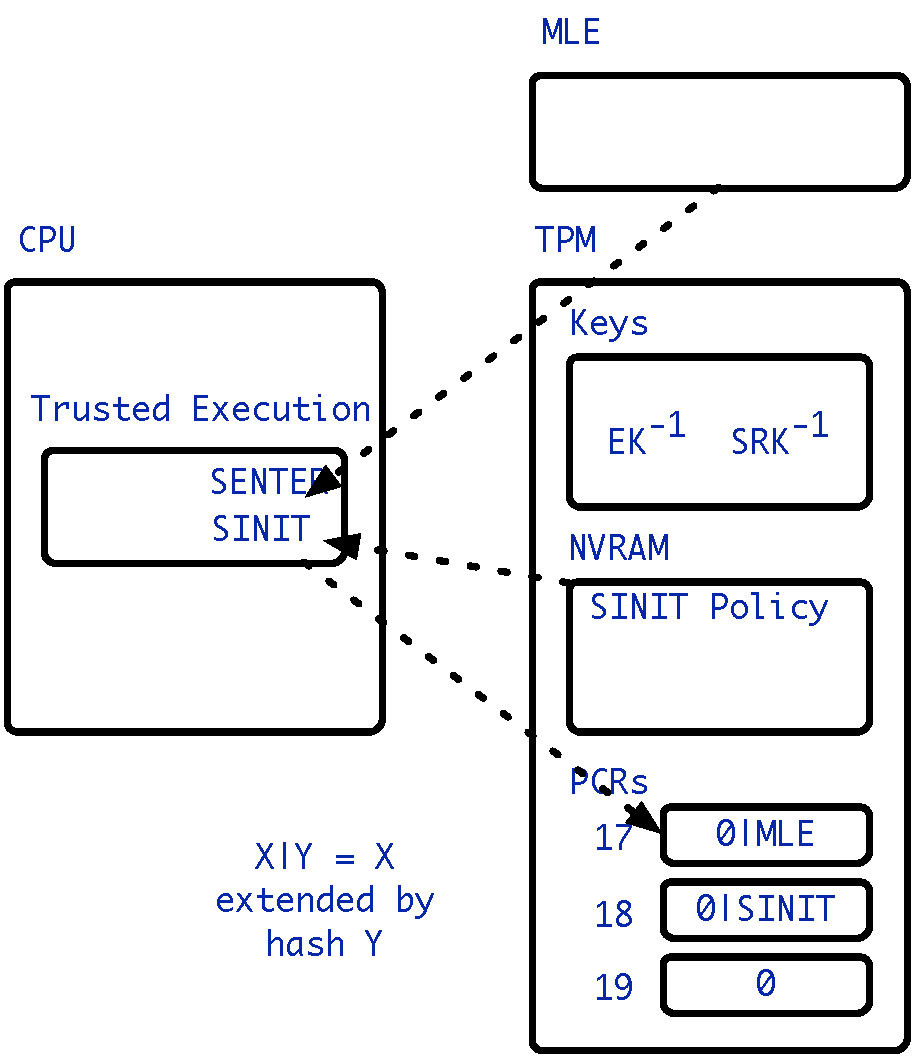
\includegraphics[width=1.0\textwidth]{figures/boot-pre-sinit.pdf}}
      \only<2>{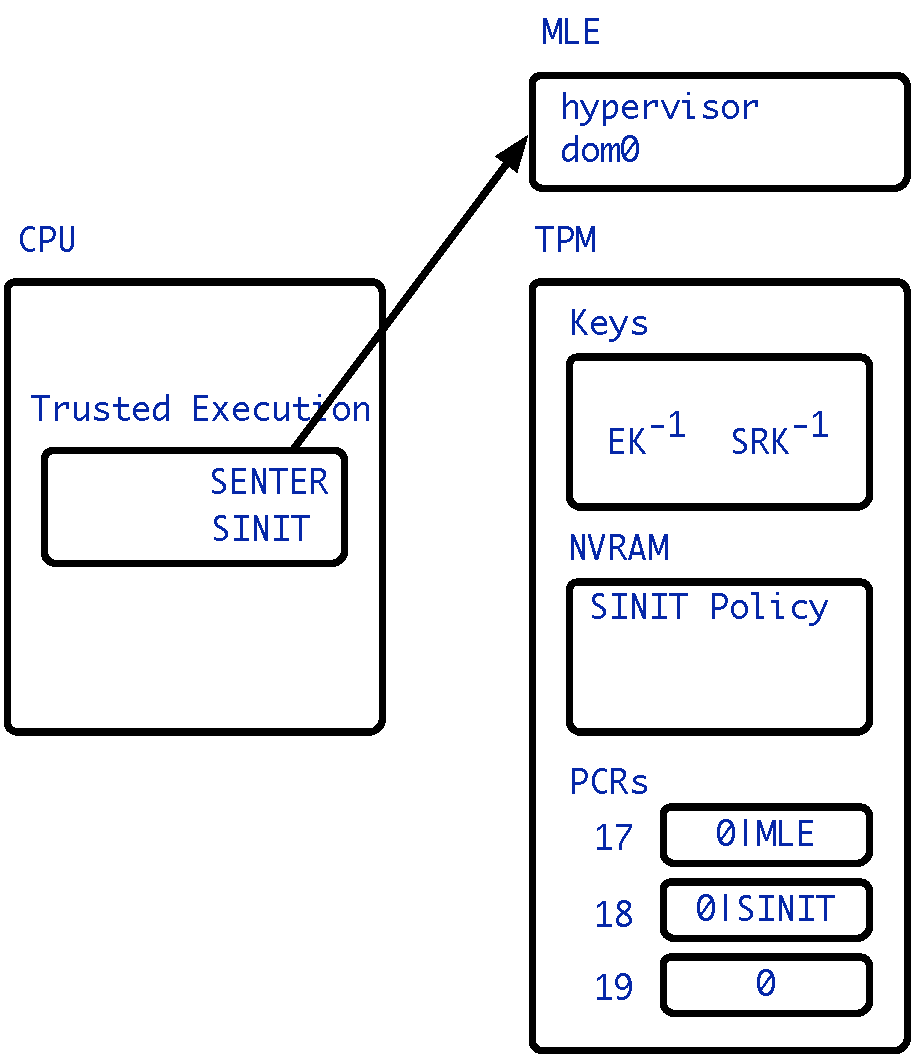
\includegraphics[width=1.0\textwidth]{figures/boot-sinit-post.pdf}}
    \end{figure}
  \end{columns}
}

\frame{\frametitle{What We Know From Good PCRs}
  \begin{itemize}
  \item \texttt{SENTER} was called --- Resetting PCR 18 starts
    measurement sequence at 0 rather than -1
  \item \texttt{SINIT} policy was measured by \texttt{SENTER} --- Only
    \texttt{SENTER} can extend PCR 18
  \item \texttt{SINIT} uses the correct policy --- PCR 18 is extended
    with \texttt{SINIT} measurement policy
  \item \texttt{SENTER} ran before \texttt{SINIT} ---
    $\extend{0}{SINIT}\neq\extend{-1}{SINIT}$
  \item \texttt{MLE} is good --- Measured by good \texttt{SINIT} into
    PCR
  \item Initial OS is good --- Measured by good \texttt{MLE} into PCR
  \end{itemize}
}

\frame{\frametitle{Boot the MLE}
  \begin{columns}[c]
    \column{.53\textwidth}
    \begin{itemize}
      \item<1-> \texttt{SENTER} starts the MLE 
        \begin{itemize}
        \item<1-> \texttt{SENTER} starts the hypervisor
        \item<1-> \texttt{SENTER} passes dom0 to hypervisor
        \item<1-> hypervisor starts dom0
        \end{itemize}
      \item<2-> dom0 constructs the Armored VP
        \begin{itemize}
        \item<2-> Measures the vTPM into the TPM
        \item<2-> Starts the vTPM
        \item<3-> Measures remaining Armored VMs into the vTPM
        \item<3-> Starts remaining Armored VMs
        \item<3-> Measures Armored application into the vTPM
        \item<3-> Starts the Armored application
        \end{itemize}
    \end{itemize}
    \column{.45\textwidth}
    \begin{figure}
      \only<1>{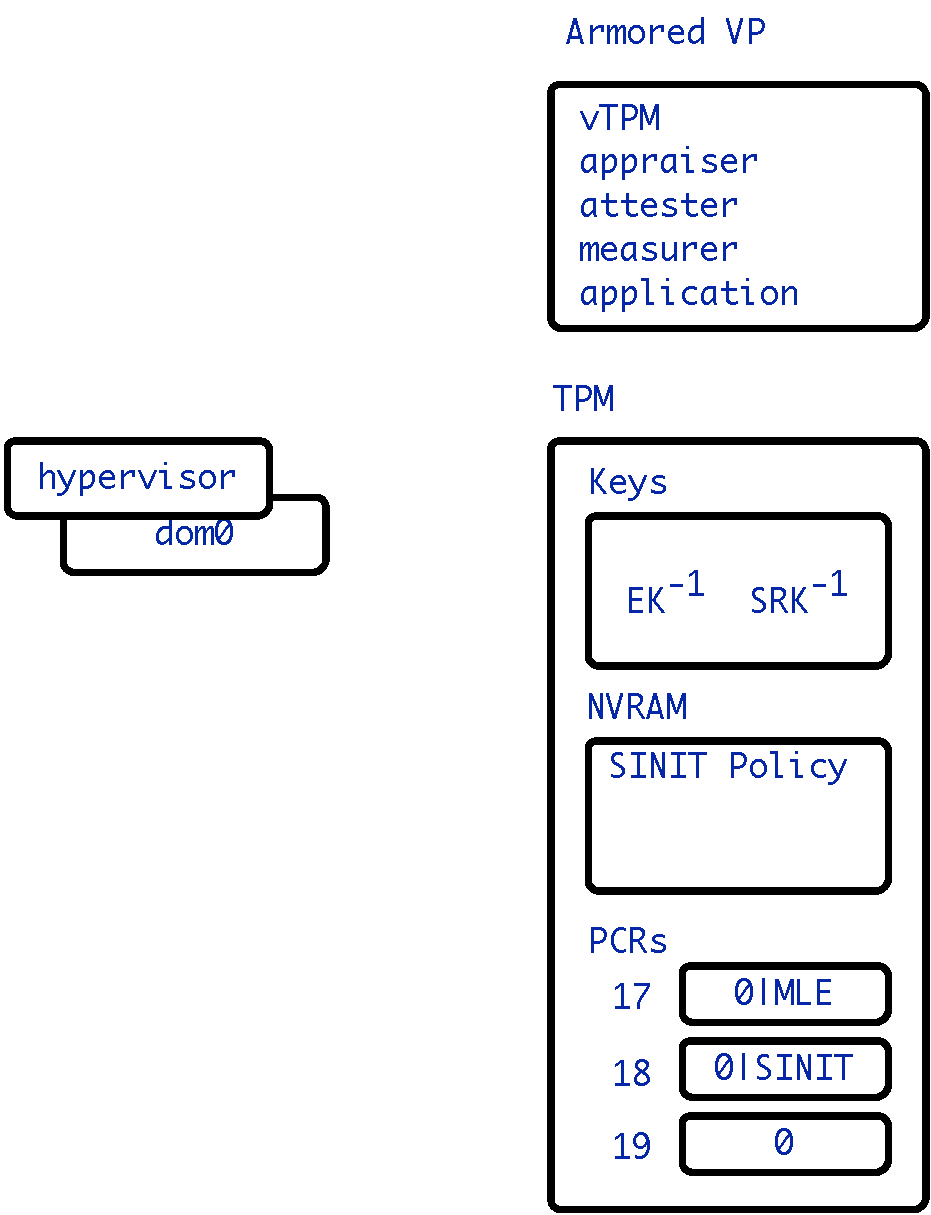
\includegraphics[width=1.0\textwidth]{figures/boot-pre-hypervisor.pdf}}
      \only<2>{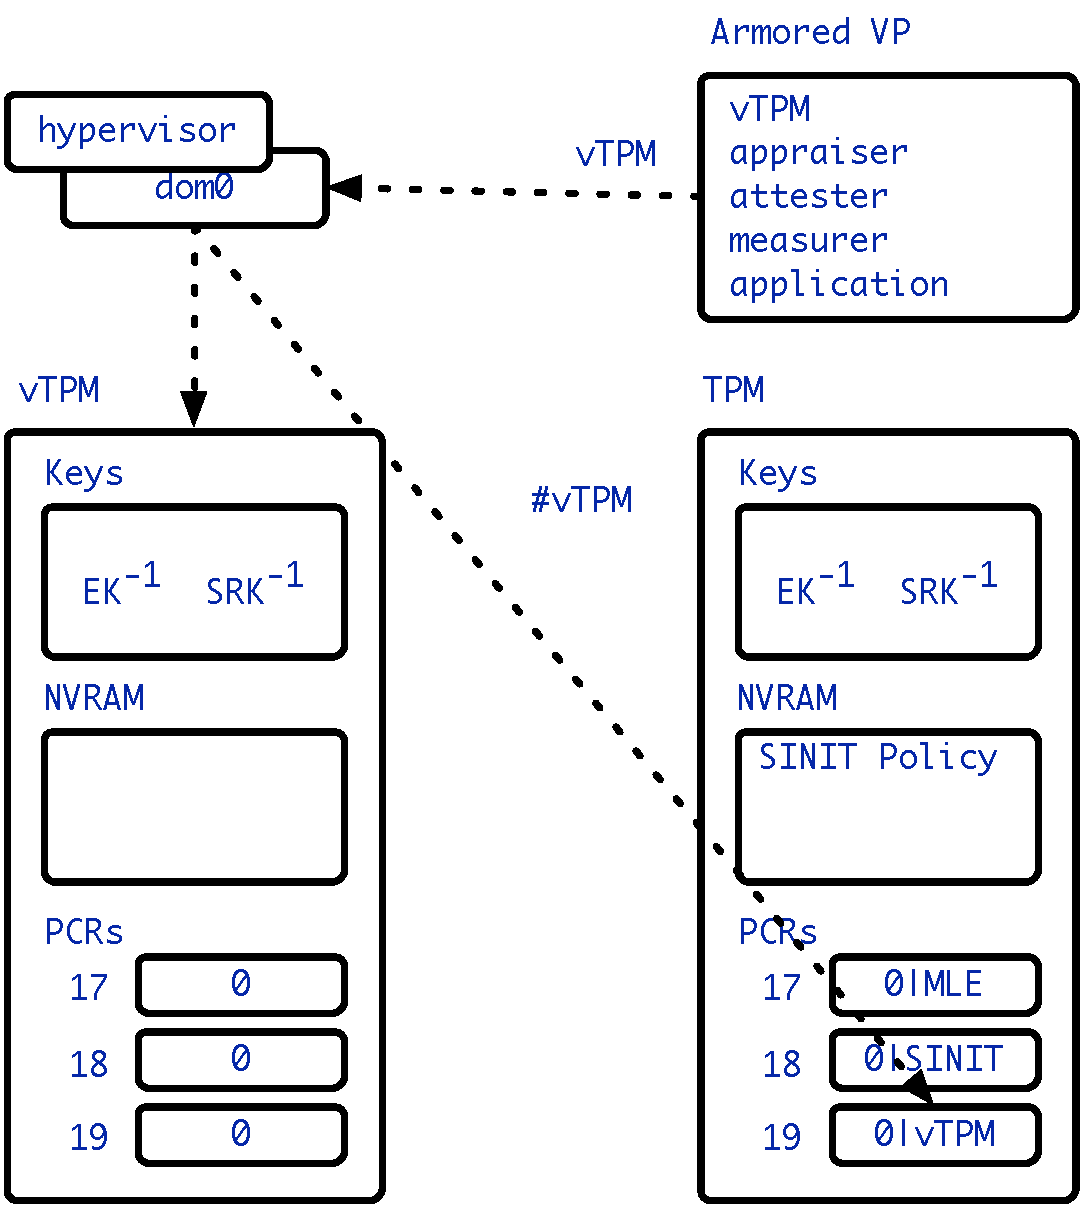
\includegraphics[width=1.0\textwidth]{figures/boot-vtpm.pdf}}
      \only<3>{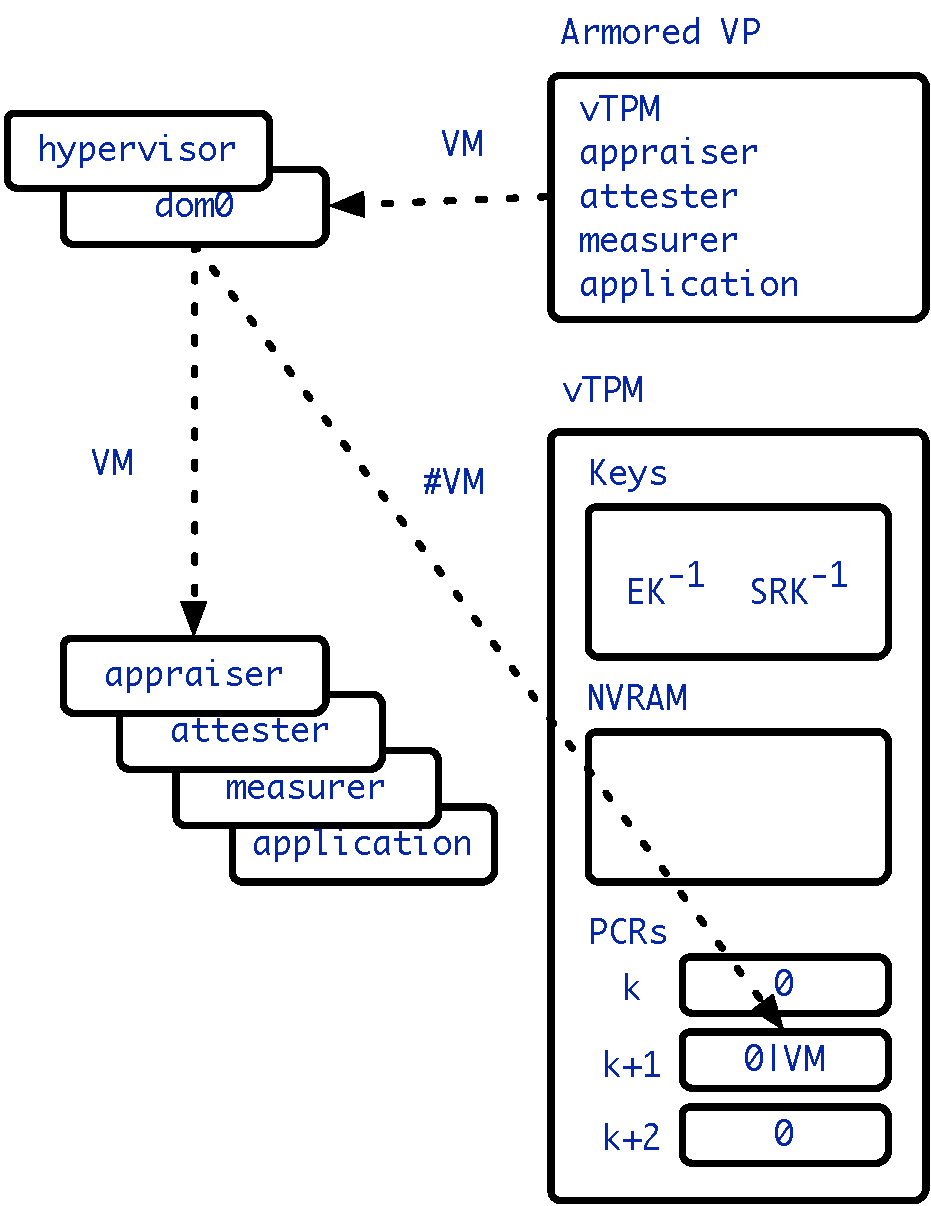
\includegraphics[width=1.0\textwidth]{figures/boot-platform.pdf}}
      \only<4>{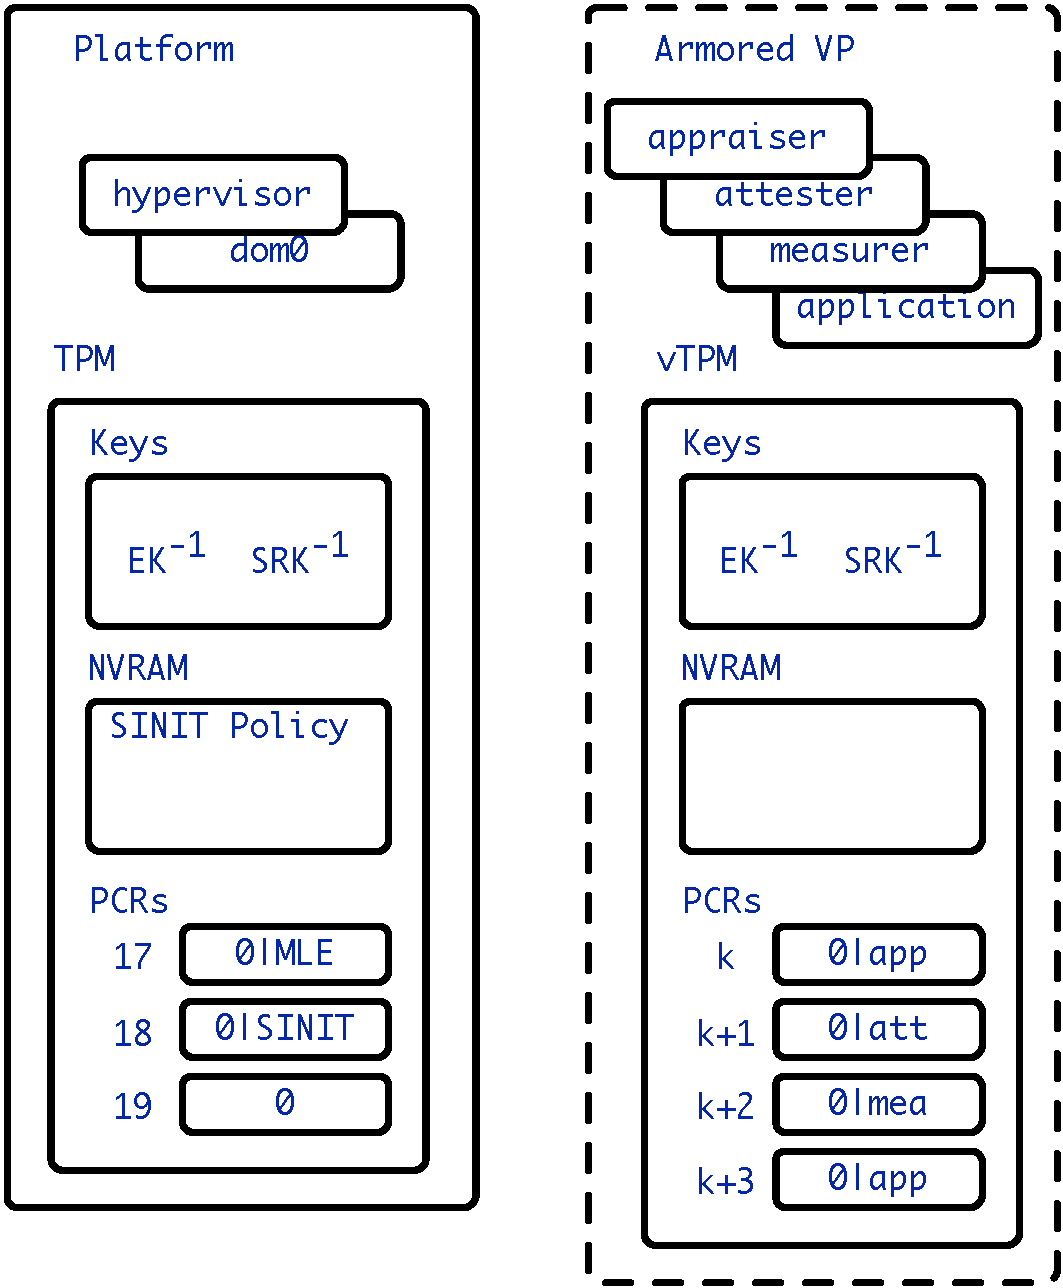
\includegraphics[width=1.0\textwidth]{figures/boot-platform-post.pdf}}
    \end{figure}
  \end{columns}
}

\frame{\frametitle{What we know from good PCRs}
  \begin{itemize}
  \item The right hypervisor and dom0 started - PCR 17 measurement and
    we trust \texttt{SENTER}, \texttt{SINIT} and \texttt{SINIT} Policy
  \item The right vTPM started - PCR 19 measurement and we trust
    \texttt{SENTER}, \texttt{SINIT}, and dom0\footnote{More work for
      vTPM startup remains}
  \item The right ArmoredSoftware components started - vTPM PCRs and
    we trust dom0 and the vTPM
  \item The right application started - vTPM PCRs and we trust dom0
    and the vTPM
  \end{itemize}
}

\frame{\frametitle{Chaining Trust (Reprise)}
  \begin{itemize}
  \item Trust is transitive
    \begin{itemize}
    \item $\trusts{x}{y} \wedge \trusts{y}{z} \Rightarrow
      \trusts{x}{z}$
    \item Construct evidence trust chains
    \item Remember ``directly observed or indirectly observed by a
      trusted third party''
    \end{itemize}
  \item Roots of Trust define the ``root'' for trust
    \begin{itemize}
    \item Use Roots of Trust to establish base for chain
    \item RTM is the Trusted Measurer
    \item RTS is the Trusted Store
    \item RTR is the Trusted Reporter (coming soon...)
    \end{itemize}
  \item Extend chains of trust by measuring before executing
  \end{itemize}
}


% \frame{\frametitle{Presentation Outline}
%   \begin{itemize}
%     \item Review access control modeling objectives
%       \begin{itemize}
%       \item modeling platform MAC
%       \item modeling local access control
%       \end{itemize}
%     \item Overview access control policy definition
%       \begin{itemize}
%       \item design and modeling assumptions
%       \item platform boot policy definition
%       \item local policy definitions
%       \end{itemize}
%     \item Overview models
%       \begin{itemize}
%       \item domain and system models
%       \item communication model
%       \item theorems and status
%       \end{itemize}
%     \item Identify next steps
%       \begin{itemize}
%       \item runtime and moving beyond the SVP line
%       \item adding M\&A detail
%       \end{itemize}
%   \end{itemize}
% }

% \frame{\frametitle{Access Control Modeling Objectives}
%   \framesubtitle{What we're about here}

%   Reporting joint work with Geoffrey Brown, Indiana University (submitted) in which
%   we verify two physical layer protocols.
%   \begin{itemize}
%     \item Biphase Mark Protocol (BMP)
%     \item 8N1 Protocol
%   \end{itemize}

% These protocols are used in data transmission for CDs, Ethernet, and Tokenring,
%       etc. as well as UARTs.  
%   \begin{itemize}
%     \item Correctness is reasonably difficult to prove due to many real-time constraints.

%     \item Many previous formal modeling/verification efforts for these protocols.
%   \end{itemize}

% }

% \frame{\frametitle{Columns and Blocks}\framesubtitle{Trying figures
%     next to lists}
%   \begin{columns}[c]
%     \column{.45\textwidth}
% %    \begin{block}{Things}
%     Some normal text goes here just for introduction
%     \begin{itemize}
%       \item Appraisal
%       \item Measurement
%       \item Attestation
%       \item vTPM
%     \end{itemize}
%     \alert{Why is this column getting higher?}\\
%     Maybe it's not\\
%     Center alignment seems best.\\
%     \alert{I like this for two column test and graphics}\\
%     Getting higher???
% %    \end{block}
%     \column{.45\textwidth}
%     \begin{figure}
%       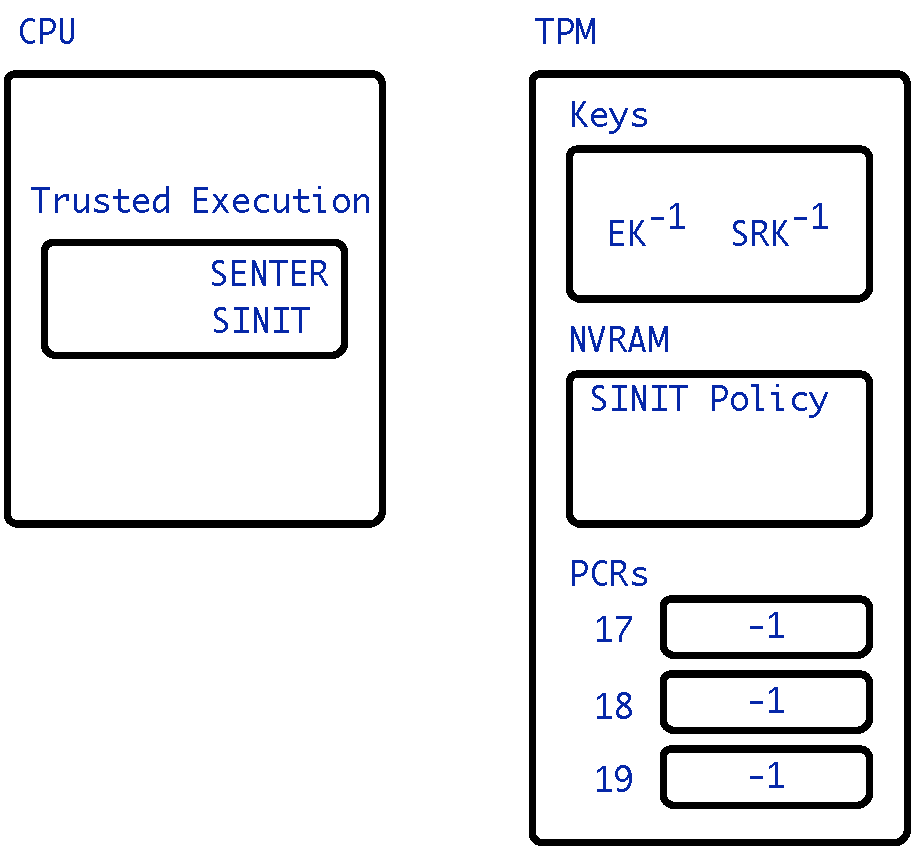
\includegraphics[width=1.0\textwidth]{figures/basic-architecture.pdf}
%     \end{figure}
%   \end{columns}
% }

% \frame[plain]{\frametitle{Big Picture}\framesubtitle{Armor Architecture}
%   \begin{figure}
% %%    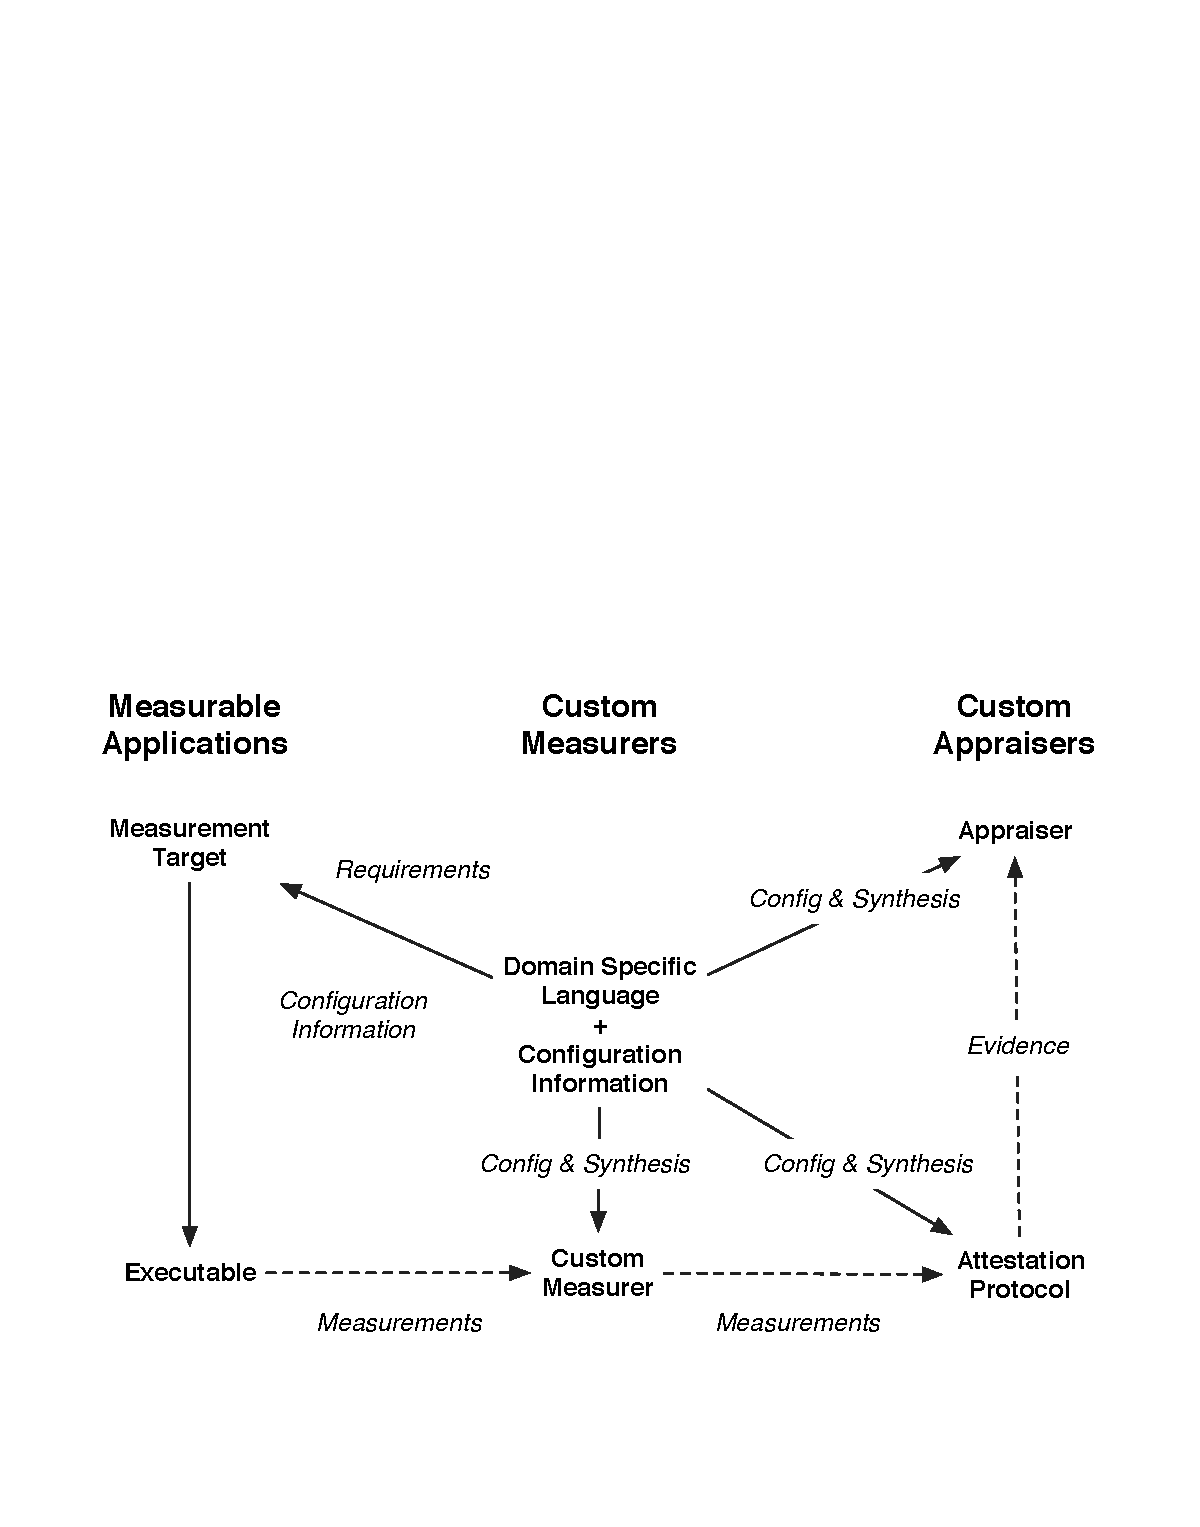
\includegraphics[height=0.70\textheight]{architecture.pdf}
%   \end{figure}
% }
    

% {\frame{\frametitle{Simple Block}
%   \begin{block}{Introduction to {\LaTeX}}
%     ‘‘Beamer is a {\LaTeX}class for creating presentations
%     that are held using a projector..."
%   \end{block}
  
%   \begin{block}{}
%     This is a definition
%   \end{block}
% }

% \frame{\frametitle{Proofs}
%   \begin{proof}[Not really a proof]
%     \begin{enumerate}
%     \item<1-3>{This is a step}
%     \item<2-3>{This is another step}
%     \item<3>{This is a third step}
%     \item<3>{This is a third step}
%     \item<3>{This is a third step}
%     \item<3>{This is a third step}
%     \end{enumerate}
%   \end{proof}
% }


% \frame{\frametitle{List with Overlays}
%   \begin{itemize}
%   \item<1-> Item 1 followed by a pause
%   \item<3-> Item 2 followed by a pause
%   \item<2-> Item 3 followed by a pause
%   \end{itemize}
% }

% \frame{\frametitle{Previous Efforts}

%   \begin{itemize}
%   \item BMP has been verified in PVS twice and required
%     \begin{itemize}
%     \item  37 invariants and 4000 individual proof directives (initially) in the
%       one effort
%     \item 5 hours just to \emph{check} the proofs in the other effort
%     \item A formal specification and verification of an independent real-time model
%       in both efforts
%     \end{itemize}
%   \item BMP has been verified in (the precursor to) ACL2 by J. Moore and required
%     \begin{itemize}
%      \item A significant conceptual effort to fit the problem in the logic, arguably
%        omitting some salient features of the model
%      \item The statement and proof of many antecedent results
%      \item J. Moore reports this as one of his ``best ideas'' in his career
%     \end{itemize}
    
%   \end{itemize}
% }

% \frame{\frametitle{Not Your Father's Theorem-Prover} 

% The verifications are carried out in the SAL infinite-state bounded model-checker
% that combines SAT-solving and SMT decision procedures to \emph{prove} safety
% properties about infinite-state models.

%   \begin{itemize}
%     \item Theorem-proving efforts took multiple engineer-months if not years to
%       complete.

%     \item Our initial effort in SAL consumed about \emph{two engineer-days}.\\
%       ...and we found a significant bug in a UART application note.
%   \end{itemize}
% }


% \frame[containsverbatim]{\frametitle{Parameterized Timing Constraints}
% SMT allows for {\color{red}\emph{parameterized}} proofs of correctness.  The following are
% example constaints from the BMP verification:
% \begin{fnverbatim}
%   TIME: TYPE = REAL;

%   TPERIOD: TIME = 16;
%   TSAMPLE: INTEGER = 23;
% {\color{red}
%   TSETTLE}: \{x: TIME |     0 <= x  
%                       AND (x + TPERIOD < TSAMPLE) 
%                       AND (x + TSAMPLE + 1 < 2 * TPERIOD)\};
% {\color{red}
%   TSTABLE}: TIME = TPERIOD - TSETTLE;
% {\color{red}  
%   ERROR}: \{x: TIME |     (0 <= x) 
%                     AND (TPERIOD + TSETTLE < TSAMPLE*(1-x)) 
%                     AND (TSAMPLE*(1+x) + (1+x) + TSETTLE < 2 * TPERIOD)\};

%   RSAMPMAX: TIME = TSAMPLE * (1 + ERROR);
%   RSAMPMIN: TIME = TSAMPLE * (1 - ERROR);
%   RSCANMAX: TIME = 1 + ERROR;
%   RSCANMIN: TIME = 1 - ERROR;
% \end{fnverbatim}
% }


% \frame[containsverbatim]{\frametitle{SRI's SAL Toolset}
%       \begin{itemize}
%         \item Parser
%         \item Simulator
%         \item Symbolic model-checker (BDDs) 
%         \item Witness symbolic model-checker 
%         \item Bounded model-checker
%         \item Infinite-state bounded model-checker
%         \item Future releases include: 
%           \begin{itemize}
%             \item Explicit-state model-checker
%             \item MDD-based symbolic model-checking
%           \end{itemize}
%       \end{itemize}
% \begin{center}
% All of which are ``state-of-the-art''
% \end{center}
% }


% \frame{\frametitle{$k$-Induction}

% Please direct your attention to the whiteboard.

% }



% \frame[label=ta]{ \frametitle{Timeout Automata\footnote{B. Dutertre
%   and M. Sorea.  Timed systems in SAL.  \emph{SRI TR}, 2004.} (Semantics)}

%   An \emph{explicit} real-time model.

%   \begin{itemize}
%   \item Vocabulary:
%   \begin{itemize}
%     \item A set of state variables.
%     \item A \emph{global clock}, $c \in \rtime$.
%     \item A set of \emph{timeout} variables $T$ such that for $t \in
%       T$, $t \in \rtime$.
%   \end{itemize}
%   \item Construct a transition system $\mean{S, \, S^0, \, \rightarrow}$:
%   \begin{itemize}
%     \item States are mappings of all variables to values.
%     \item Transitions are either \emph{time transitions} or
%       \emph{discrete transitions}.
%       \begin{itemize}
%         \item Time transitions are enabled if the clock is less than
%           all timeouts.  Updates clock to least timeout.
%         \item Discrete transitions are enabled if the clock equals
%           some timeout.  Updates state variables and timeouts.
%       \end{itemize}
%   \end{itemize}
%   \end{itemize}
% }

% \frame[containsverbatim]{\frametitle{Disjunctive Invariants} Even with $k$-induction, getting a
%   sufficiently strong invariant is still hard!  \emph{Disjunctive invariants} help.
%   A disjunctive invariant can be built iteratively from the counterexamples returned
%   for the hypothesized invariant being verified.

% \begin{fnverbatim}
%   t0:  THEOREM system |- 
%          G(   (    (phase = Settle) 
%                AND (rstate = tstate + 1) 
%                AND (rclk - tclk - TPERIOD > 0) 
%                AND (tclk + TPERIOD + TSTABLE - rclk > 0))
%            OR
%               (    (phase = Stable) 
%                AND (rstate = tstate + 1) 
%                AND (rclk - tclk - TSETTLE > 0) 
%                AND (tclk + TPERIOD - rclk > 0)  
%                AND (rdata = tdata))

%                         .
%                         .
%                         .
% \end{fnverbatim}
% }

\bibliography{sldg}

\end{document}

